\mychapter{Temporário}{cap:temporario} \lhead{Temporário}


\section{Materiais e Métodos} %Remove later
 \begin{itemize}
    \item Identificar a partir do Datasheet do Manipulador informações sobre a física, tais como massa de cada elo, limitações das juntas e etc.
    \item Modelar o robô em software de CAD 3D a fim de obter informações sobre a inércia do robô e distribuição de massa.
    \item Através do modelo esquemático do robô, construir a matriz de Transformação homogênea
    \item Calcular a matriz Jacobiana do Robô, a fim de encontrar as singularidades de posição possíveis para o manipulador
    \item Produzir uma rota esperada utilizando cinemática inversa e evitando pontos de singularidade.
    \item Utilizar as equações de Euler-Lagrange para construir o modelo dinâmico, utilizando forças de inércia, efeitos de rotação, efeito de coriolis e gravitacional. Sendo estes calculados através das informações obtidas nos passos anteriores.
    \item Utilizar o método de Ziegler–Nichols para obter coeficientes para o controlador PID
    \item Realizar simulação aplicando o modelo elaborado, controlador calculado e restrições dos motores.
 \end{itemize}

\section{Testes Latex}  
\begin{equation}
{}^{n - 1}T_n  =
\operatorname{Rot}_{x_{n-1}}(\alpha_{n-1}) \cdot \operatorname{Trans}_{x_{n-1}}(a_{n-1}) \cdot \operatorname{Rot}_{z_{n}}(\theta_n) \cdot \operatorname{Trans}_{z_{n}}(d_n)
\end{equation}

\begin{equation}
T_{0,n} = 
\begin{pmatrix}
R_{1,1} & R_{1,2} & R_{1,2} & x \\
R_{2,1} & R_{2,2} & R_{2,2} & y \\
R_{3,1} & R_{3,2} & R_{3,2} & z \\
0 & 0 & 0 & 1
\end{pmatrix}
\end{equation}


\begin{equation}
M_{n-1,n} =  \left[ \begin{array}{ccc|c} R_{xx} & R_{xy} & R_{xz} & T_x \\ R_{yx} & R_{yy} & R_{yz} & T_y \\ R_{zx} & R_{zy} & R_{zz} & T_z \\
\hline
0 & 0 & 0 & 1 \end{array}\right]
\end{equation}

\begin{figure}[htbp]
    \centering
        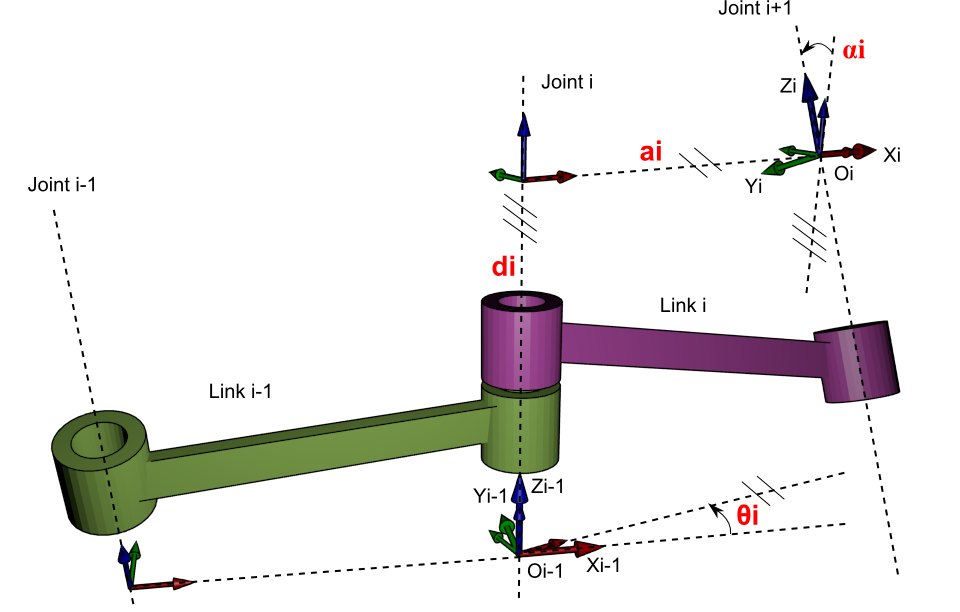
\includegraphics[width=0.95\textwidth]{imagens/dh.png}
    \caption{Minha primeira figura.}
    \label{fig:Figura1}
\end{figure}

\begin{equation}
M_{i,k}= M_{i,j} M_{j,k}
\end{equation}


\begin{algorithm}[H]
\caption{Calculate $y = x^n$}
\begin{algorithmic}
\REQUIRE $n \geq 0 \vee x \neq 0$
\ENSURE $y = x^n$
\STATE $y \leftarrow 1$
\IF{$n < 0$}
\STATE $X \leftarrow 1 / x$
\STATE $N \leftarrow -n$
\ELSE
\STATE $X \leftarrow x$
\STATE $N \leftarrow n$
\ENDIF
\WHILE{$N \neq 0$}
\IF{$N$ is even}
\STATE $X \leftarrow X \times X$
\STATE $N \leftarrow N / 2$
\ELSE[$N$ is odd]
\STATE $y \leftarrow y \times X$
\STATE $N \leftarrow N - 1$
\ENDIF
\ENDWHILE
\end{algorithmic}
\end{algorithm}